%*******************************************************************************
%*********************************** First Chapter *****************************
%*******************************************************************************

\chapter{Introduction}  %Title of the First Chapter

\ifpdf
    \graphicspath{{Chapter1/Figs/Raster/}{Chapter1/Figs/PDF/}{Chapter1/Figs/}}
\else
    \graphicspath{{Chapter1/Figs/Vector/}{Chapter1/Figs/}}
\fi

Gallium nitride \nomenclature[z-GaN]{GaN}{Gallium Nitride} (GaN) has been termed the 'most important semiconductor material since silicon' \cite{Humphreys2008}, and indeed the influence of this incredible material and it's associated alloys (termed III-nitrides) is pervasive in modern society. The impact of III-nitride materials is perhaps best evidenced by the global transition from traditional lighting sources to semiconductor lighting solutions based on III-nitride materials. Since the first demonstration of a high-brightness blue light emitting diode \nomenclature[z-LED]{LED}{Light-Emitting Diode} (LED) in 1991 by Shuji Nakamura \cite{Nakamura1991}, the widespread use of LEDs for general lighting purposes has blossomed into a multi-billion pound industry. The extraordinary optical properties of III-nitride materials have enabled their application outside of the lighting industry: the development of III-nitride based lasers has found applications in telecommunications \cite{Najda2015}, medicine \cite{BerlienBreuerMuellerEtAl2012} and data storage . Furthermore, III-nitride optical emitters have been used as single photon sources \nomenclature[z-SPS]{SPS}{Single Photon Source} (SPSs) which have applications in cryptography for secure communications \cite{Kako2006}.
\\The optoelectronic properties of III-nitride materials are somewhat astonishing: GaN suffers from a defect density several orders of magnitude higher than other optically active semiconductor materials such as gallium arsenide \nomenclature[z-GaAs]{GaAs}{Gallium Arsenide} (GaAs) \cite{Bennett2010b} yet is still optically active. Despite this, the effects of defects originating from the heteropitaxial growth of GaN are clearly deleterious when considering III-nitride device operation. 
This work aims to explore the manner in which the microstructural properties of photonic III-nitride devices affect their performance by combining multiple microscopy techniques, an approach we term 'multi-microscopy', thus allowing us to link specific structural features with emissive properties at the device level. The experimental research in this thesis is separated into four main sections. 
\\The first section details the investigation of inhomogeneous electroluminescence \nomenclature[z-EL]{EL}{Electroluminescence} (EL) of indium gallium nitride (InGaN) quantum well (QW) LEDs. By employing the use of scanning probe techniques, electron microscopy and spectroscopy the underpinning cause of LED behaviour was elucidated and reported.
\\The second section involves microscopy-based investigation into the mechanisms behind incomplete etching in the fabrication of III-nitride based microdisk cavities and the effect of this issue on the overall optical performance of these cavities
\\The third section describes the microscopy of one dimensional \nomenclature[z-1-D]{1-D}{One-Dimensional} (1-D) photonic crystal cavity (PCC) 'nanobeam' cavities. The intrinsic resistance of III-nitride based materials can often result in improperly etched features, which can results in high optical losses in cavities. This section concerns the use of tomographic techniques such as electron tomography \nomenclature[z-ET]{ET}{Electron Tomography} (ET) and focussed ion beam tomography \nomenclature[z-FIBT]{FIBT}{Focussed Ion Beam Tomography} (FIB-T) to investigate the effect of these issues on the emission of III-nitride nanobeam cavities. 

%********************************** %First Section  **************************************
\section{III-Nitride Material Properties } %Section - 1.1 

\subsection{Crystal Structure}
\label{section1.1.1}

GaN can crystallise into two distinct crystal structures: hexagonal (wurtzite) and cubic (zinc blende and rock salt). Under ambient conditions, wurtzite GaN is the most commonly studied form as it is the most structurally stable. Thus, the work discussed in this thesis concerns wurtzite III-nitrides. A schematic of a wurtzite III-nitride crystal structure is shown in Fig.\ref{1.1} and consists of stacked hexagonal close-packed planes following an ABABAB stacking sequence. Atoms of the respective elements are tetrahedrally bonded to one another. However, in the case of III-nitrides this structure deviates from ideal tetrahedral bonding and results in a non-zero dipole moment for each unit cell which will be discussed in the following sections.
\\ A 4-index Miller-Bravais notation (hkil) is used to denote the crystal planes where the index {\it i} is defined by the relation:

\begin{equation}
 i = -(h+k)
 \end{equation}
\\
 
The crystallographic planes (0001), (1-100) and (11-20) shown in Fig.\ref{1.1} are often termed the {\it c}, {\it m} and {\it a}-planes in the literature. The fundamental unit cell of the wurtzite GaN crystal structure and its associated lattice parameters \textbf{a} and \textbf{c} is shown in Fig.\ref{1.2}

\begin{figure}[h]
	\centering
	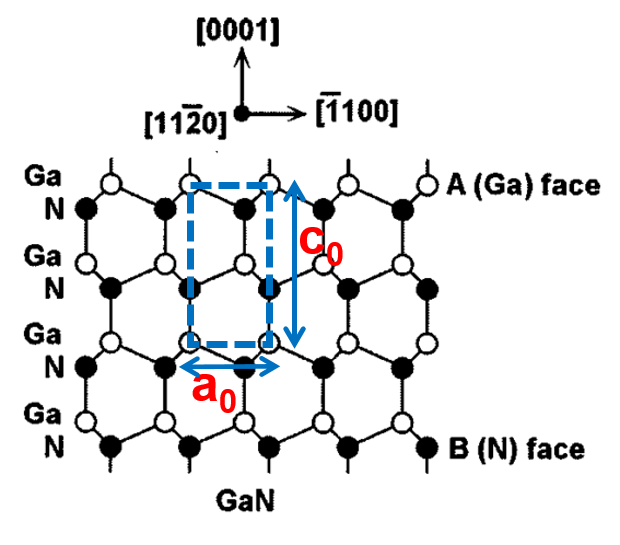
\includegraphics[width=0.5\textwidth]{Figs/Ch1/unit_cell.png}
	\caption {Unit cell (dashed line) for GaN crystal structure and lattice parameters $\mathbf{a_{0}},\mathbf{c_{0}}$. Adapted from \cite{Yu1999}}
	\label{1.2}
\end{figure}
\FloatBarrier

Other members of the III-nitride materials such as indium nitride \nomenclature[z-InN]{InN}{Indium Nitride} (InN) or aluminium nitride \nomenclature[z-AlN]{AlN}{Aluminium Nitride} (AlN) have different lattice parameters due to the differing atomic radii of aluminium and indium relative to gallium.

\begin{table}[!htb]
	\centering
	
	\begin{tabular}{ccc}
		Alloy & \textbf{a} (\si{\angstrom}) at T = 300K & \textbf{c} (\si{\angstrom}) at T = 300K \\
		%heading
		\hline\hline
		GaN   & 3.189   & 5.185   \\
		InN   & 3.545   & 5.703   \\
		AlN   & 3.112  & 4.982  \\ 
		\hline
	\end{tabular}
	\caption{Room temperature lattice parameters for GaN, InN and AlN \cite{Vurgaftman2003}.}
	\label{tab1.1}
\end{table}

III-nitride photonic devices are often heterostructures consisting of ternary alloys the materials shown in Table~\ref{tab1.1}. Lattice parameters of a relaxed ternary alloy $A_{x}B_{1-x}N$ can be estimated using Vegard's law \cite{Vickers2003}:

\begin{equation}
\mathbf{a} = x \mathbf{a}_{AN} + (1-x)\mathbf{a}_{BN}
\end{equation}

\begin{equation}
\mathbf{c} = x \mathbf{c}_{AN} + (1-x)\mathbf{c}_{BN}
\end{equation}

Typical indium compositions for blue LEDs range between 15-20 $\%$, which leads to a considerable lattice mismatch of approximately 2 $\%$, resulting in considerable amounts of strain in these GaN/InGaN heterostructures.

\subsection{Band Structure} 
\label{section1.1.2}

One of the principal driving factors behind the interest in III-nitrides for photonic devices is their direct bandgap which collectively spans the visible spectrum and beyond. The bandgap of III-nitride binary alloys is given below in Table.\ref{tab1.2}.

\begin{table}[!htb]
	\centering
	\begin{tabular}{cc}
		Alloy & Bandgap (eV) \\
		%heading
		\hline\hline
		GaN   & 3.51 \\
		InN   & 0.78 \\
		AlN   & 6.25  \\ 
		\hline
	\end{tabular}
	\caption{Direct bandgaps of GaN, InN and AlN \cite{Vurgaftman2003}.}
	\label{tab1.2}
\end{table}

Ternary alloying modifies the bandgap as shown in Fig.\ref{bgap}. In theory the entire range of 0.78-6.25 eV is accessible through alloying, though material limitations reduce the full effective range for III-nitride devices \cite{Scholz2012}.

\begin{figure}[h]
	\centering
	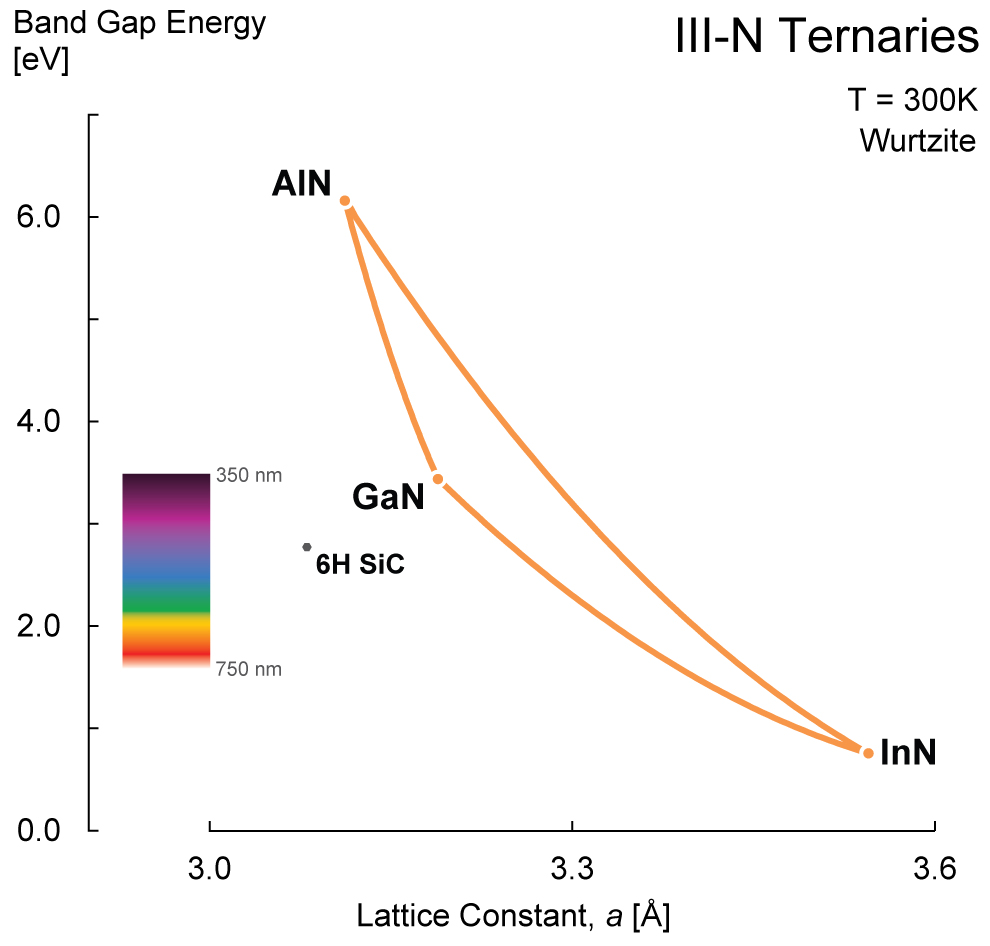
\includegraphics[width=0.7\textwidth]{Figs/Ch1/III-N-Ternaries-update.jpg}
	\caption {Bandgap at room temperature for III-nitride materials with the visible spectrum shown on the left. Courtesy of K. Montgomery.}
	\label{bgap}
\end{figure}
\FloatBarrier

The bandgap of a ternary alloy $A_{x}B_{1-x}N$ is given by a modified Vegard's Law:

\begin{equation}
E_{g} = x E_{g}^{AN} + (1-x)E_{g}^{BN}-x(1-x)C
\end{equation}

Where C is a bowing parameter which accounts for deviation from a linear relation between ternary alloy composition and bandgap energy. The value of the InGaN bowing parameter has been widely debated in the literature due to the lack of a reliable value for the bandgap energy for InN \cite{Vurgaftman2003}. Although the current value of 1.4 eV is reported, there are also suggestions the bowing parameter may be composition dependent \cite{Wu2002,McCluskey2003,Moses2010}.\\
In considering the optical properties of III-nitride materials it is also important to consider the effects of impurities and defects. Crystal disorder introduces further energy states which would be 'forbidden' in an ideal crystal lattice leading to an effective 'smearing' of the bandgap. Sub-bandgap absorption can occur due to the introduction of these defective states. The smearing out of the absorption edge of the material is known as the 'Urbach tail', and can be a highly deleterious source of loss in III-nitride cavity structures \cite{Puchtler2015}. 

\subsubsection{Quantum Confinement Effects}

The first prototype high-brightness blue III-nitride LED consisted of a GaN {\it p-n} junction, or a 'homojunction' \cite{Nakamura1991}, however modern LED structures consist of heterostructures known as quantum wells. QWs consist of a thin layer of low bandgap material between two quantum barriers with a higher bandgap. Carriers in the low bandgap material are effectively confined in one direction, hence the term 'quantum well'. This confinement leads to the discretisation of the carrier wavefunctions within the well, as shown schematically in Fig.\ref{QW}.

\begin{figure}[h]
	\centering
	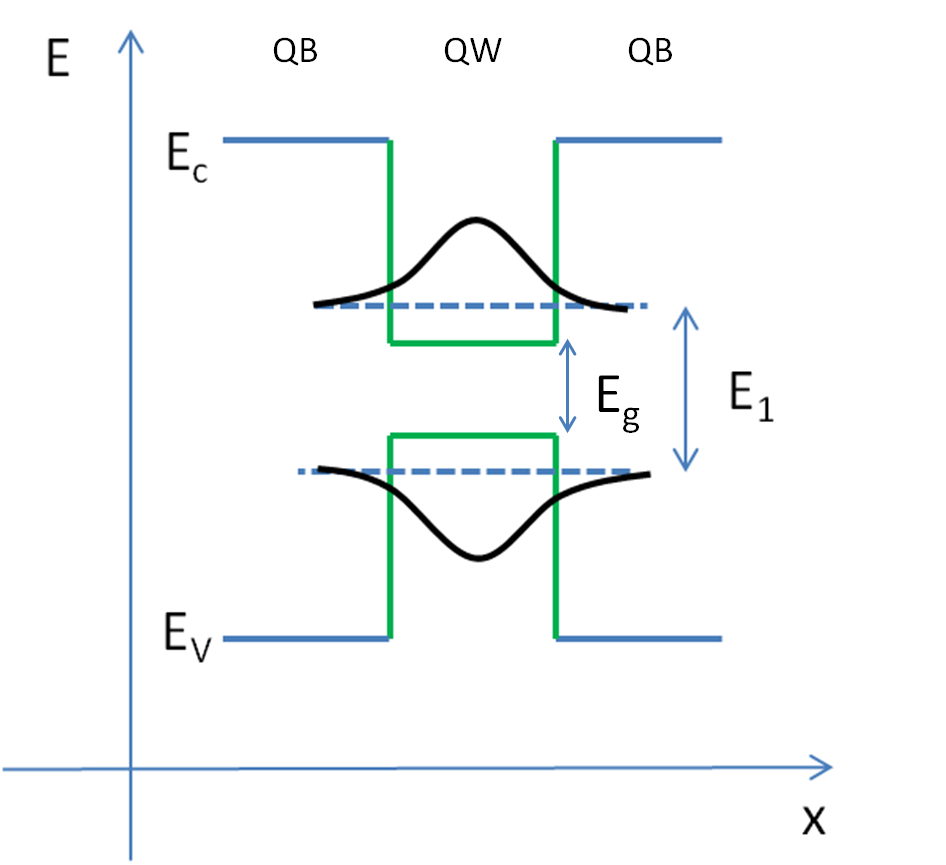
\includegraphics[width=0.5\textwidth, trim = 4 4 4 4 , clip]{Figs/Ch1/BandstructureQW.png}
	\caption {Band diagram of a quantum well. The bandgap of the well material is denoted $E_{g}$, the energy of the ground state transition is denoted $E_{1}$ and the conduction and valence bands are denoted $E_{c},E_{v}$ respectively \cite{Ren2015}.}
	\label{QW}
\end{figure}
\FloatBarrier

Thus the energy of the transition in the QW is given by the following relation:

\begin{equation}
h\nu = E_{1}-E_{ex}
\end{equation}

where $E_{1}$ is the energy of the ground state transition and $E_{ex}$ is the exciton binding energy. For an infinite potential well of thickness L, the ground state $E_{1}$ is given by:

\begin{equation}
E_{1}=\frac{\hbar^{2}\pi_{2}}{2m^{*}L^{2}}
\end{equation}

where $\hbar$ is the reduced Plank constant, $m^{*}$ is the carrier effective mass. As such, the energy of the optical transition can be related to the thickness of the well.





\subsection{Built-in Fields} 
\label{section1.1.3}
III-nitride materials in wurtzite structure are termed 'polar' materials, due to the fact they exhibit a spontaneous polarisation field \cite{Ambacher2002}. This occurs due to III-nitride bonding structure deviating from an ideal tetrahedral structure along the (0001) axis along the crystal, combined with the ionicity of the bond \cite{Ren2015}. This deviation causes each unit cell to possess a non-zero dipole moment along the principal axis of the tetrahedral bonding structure, resulting in an overall spontaneous polarization in the crystal. As the III-nitride wurtzite structure is non-centrosymmetric, the direction of the polarization depends on whether the crystal exhibits (+ {\it c}) or (-{\it c}) polarity, as shown in Fig.\ref{1.3}

\begin{figure}[h]
	\centering
	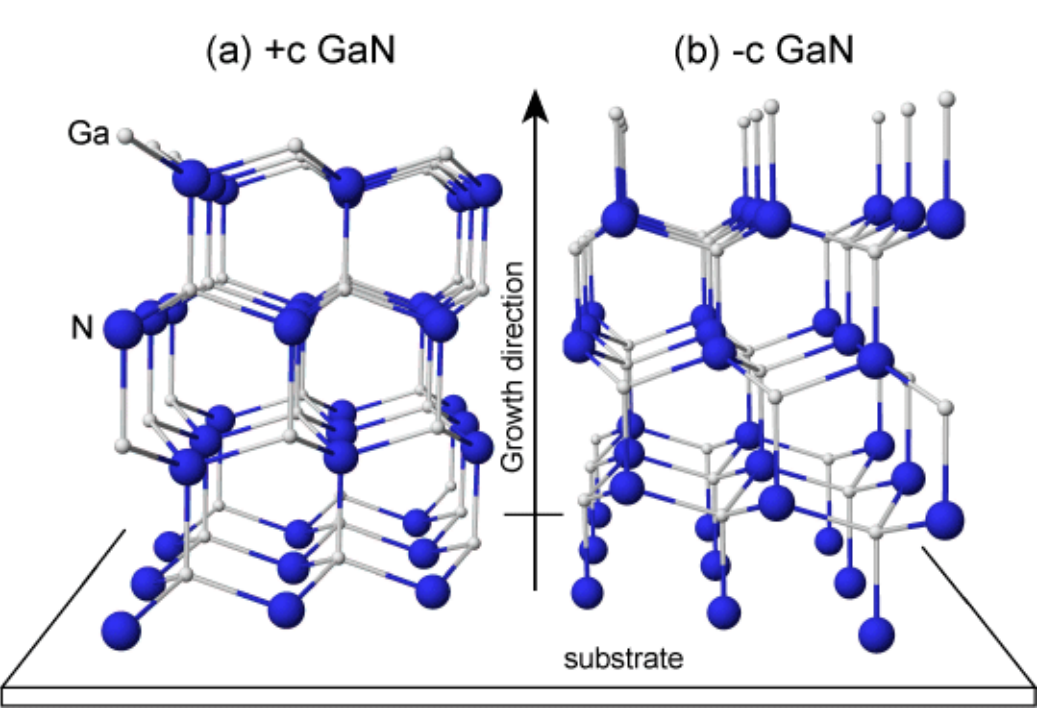
\includegraphics[width=0.5\textwidth]{Figs/Ch1/p2.png}
	\caption {Illustration of Ga-face (+ {\it c}) and N-face (-{\it c}) GaN wrutzite crystal exhibiting polarity along the {\it c}-axis \cite{Sumiya2004}.}
	\label{1.3}
\end{figure}
\FloatBarrier

This non-zero dipole moment is particularly strong for III-nitrides relative to other III-V semiconductors due to the strong electronegativity and small size of nitrogen compared to other group V elements, resulting in a metal-nitrogen bond with greater ionicity than other III-V bonds \cite{wood2007polarization}. Fig.\ref{1.4} shows a GaN unit cell with lattice parameters {\textbf {\it c}} and \textbf{\it a} denoted.

\begin{figure}[h]
	\centering
	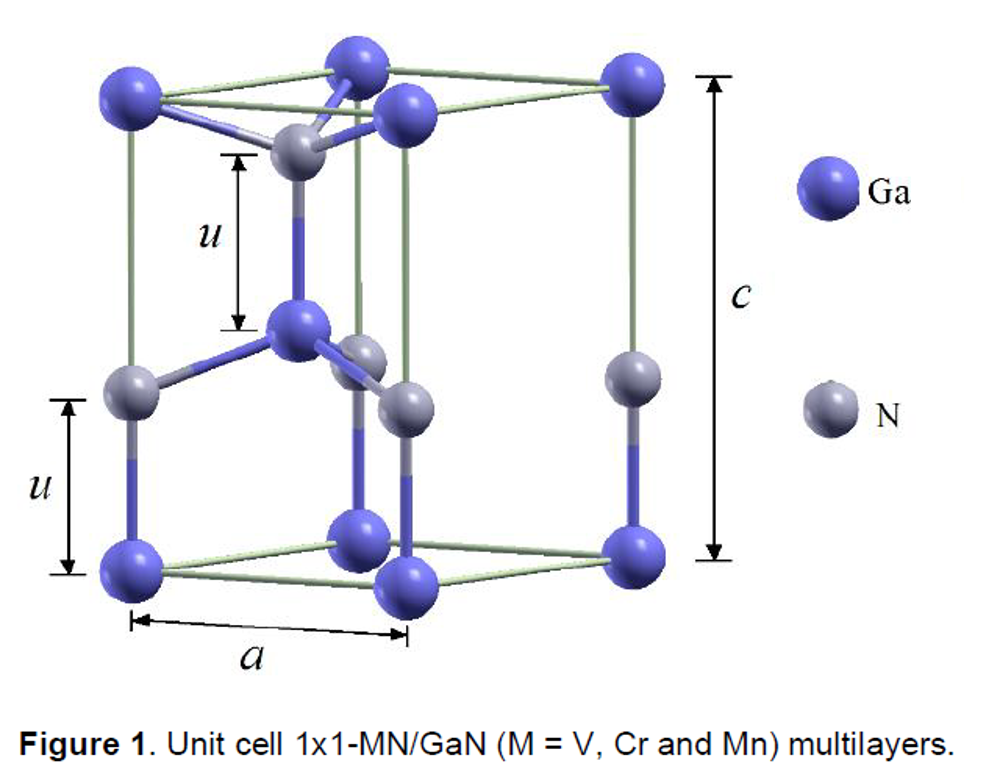
\includegraphics[width=0.5\textwidth]{Figs/Ch1/2unit.png}
	\caption {GaN unit cell with lattice parameters \textbf{\it c} and \textbf{\it a} \cite{Miguel2014}}
	\label{1.4}
\end{figure}
\FloatBarrier 

If all nearest neighbour bond lengths are equal, an ideal hexagonal closed packed crystal exhibiting zero spontaneous polarisation would have a ratio of lattice parameters denoted by:

\begin{equation}
\frac{c}{a}= (\frac{8}{3})^{0.5} = 1.63299
\end{equation} 

The degree of spontaneous polarisation observed in III-nitride materials is thus determined by the amount their lattice parameter ratio deviates from this ideal value. The values for bulk III-nitride materials are given in Table.\ref{tab1.3}. 

\begin{table}[!htb]
	\centering
	\label{tab1.1}
	\begin{tabular}{cc}
		\textbf{Alloy} &  $\mathbf{\frac{c}{a}}$ \\
		%heading
		\hline\hline\\
		GaN   & 1.6259      \\
		InN   & 1.6116     \\
		AlN   & 1.6010   \\ 
		\hline
	\end{tabular}
	\caption{Bulk $\frac{c}{a}$ ratios for GaN, InN and AlN \cite{Ren2015}.}
	\label{tab1.3}
\end{table}

A lower $\mathbf{\frac{c}{a}}$ ratio indicates a higher angle between the three bonds at the base of the tetrahedral bonding structure, resulting in a lower compensation polarisation along the (0001) axis and a higher spontaneous polarisation. Thus according to Table.\ref{tab1.2} the strongest spontaneous polarisation is observed in AlN and the weakest in GaN.\\
It is important to note that materials which exhibit spontaneous polarisation also exhibit piezoelectric polarisation \cite{Ambacher2002}. Strain experienced by the material results in the distortion in of the crystal lattice, which can either alleviate or exacerbate the deviation from the ideal tetrahedral structure resulting in an additional polarisation. This piezoelectric polarization is a crucial consideration in III-nitride devices which often consist of QW heterostructures: lattice mismatches with underlying layers result in the expansion or contraction of III-nitride films. Interestingly two different polarisation configurations are obtained for AlGaN and InGaN coherently strained to GaN. In the case of InGaN the piezoelectric field acts against the spontaneous field, whilst the opposite is true for AlGaN strained to GaN. Within the context of visible light LEDs, InGaN containing QWs are dominated by the piezoelectric contribution to the polarization fields \cite{Fiorentini1999} due to the sizeable lattice mismatch between GaN and InN ($~11\%$) \cite{Chichibu2006}.

\subsubsection{The Quantum Confined Stark Effect}

As previously discussed, III-nitride photonic devices often make use of heterostructures known as quantum wells, which enhance radiative efficiency by confining carrier wavefunctions over a range of several nanometres. Given the presence of built-in fields in III-nitride materials, it is important to consider the effect polarisation fields will have on the band structure and thus optical properties of quantum wells as shown in Fig.\ref{1.5}

\begin{figure}[h]
	\centering
	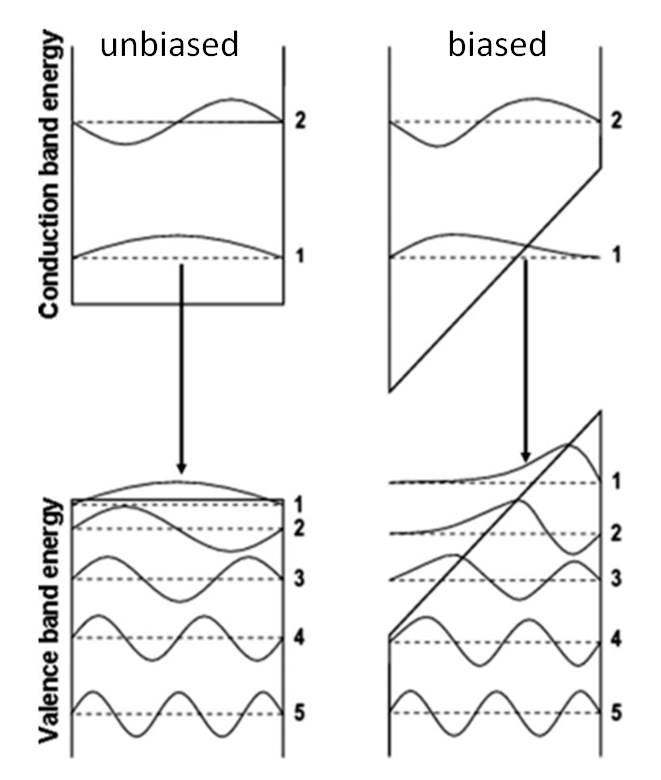
\includegraphics[width=0.5\textwidth]{Figs/Ch1/QCSE.png}
	\caption {Unbiased and biased quantum well energy levels with associated carrier wavefunctions. Under an applied field the overlap between the electron and hole carrier wavefunctions is reduced \cite{Ryou2009}.}
	\label{1.5}
\end{figure}
\FloatBarrier 

The transition from a rectangular to a 'sawtooth'-shaped potential well results in the reduction in energy of the optical transition, meaning the photons emitted from the QW are red-shifted. However, as the carrier density within the QW is increased, by either optical or electrical injection, the polarization fields are effectively screened resulting in a carrier density-dependent optical transition energy.\\
A further effect of the polarization fields is to spatially separate the carrier wave functions, thus reducing their overlap as shown in Fig.\ref{1.5}. This results in a reduced probability for the radiative recombination carriers thus reducing the efficiency of III-nitride QW emitters.
\subsection{Defects in III-nitrides}  %Section - 1.4 
\label{section1.1.4}
Many issues with III-nitride based optoelectronic devices arise from the high defect densities present. Dislocation densities tend to be several orders of magnitude higher for nitride devices relative to other III-V materials due to the lack of a low cost, widely-available lattice matched substrate \cite{Bennett2010b}. Lattice mismatch and alloy-dependent growth temperatures results in the presence of imperfections in the crystal structure of the epitaxial film known as defects. These defects can result in perturbations to the electrical and optical properties of an 'ideal' crystal, and are often classified based on their spatial dimensions. 0-D defects are often referred to as point defects, 1-D defects are commonly termed linear defects or dislocations, 2-D defects are known as planar defects or stacking faults, and there are a variety of 3-D defects known as volume defects.

\subsubsection{0-D Defects}
Point defects exist in four main forms, shown in Fig.\ref{1.6}. Vacancies, where an atom is missing from the lattice, and self-interstitial point defects are termed 'native defects': there is no inclusion of foreign atoms. These two types of intrinsic point defects are shown in Fig.\ref{1.6} a) and b) respectively.\\ 
In the case of GaN, three types of vacancies can exist: gallium vacancies, nitrogen vacancies and divacancies. The gallium vacancy ($V_{Ga}$) which has a low formation energy in {\it n}-type GaN and is acceptor-like, this vacancy has a low migration barrier. Due to this low migration energy, it is expected that gallium vacancies form complexes with more stable defects. Gallium vacancies and associated complexes are thought to be the cause of yellow luminescence observed in {\it n}-type GaN. Nitrogen vacancies initially attracted a large amount of interest due to the common belief that their energy levels were close to or within the conduction band. Due to this, the {\it n}-type conductivity of undoped GaN was attributed to nitrogen vacancies.  However, calculations have shown the thermal equilibrium of nitrogen vacancies to be too low to account for the observed conductivity. Nitrogen vacancies are also expected to have relatively low migration barriers, indicating complexes involving more stable defects may occur during high-temperature growth or annealing, especially in {\it p}-type GaN \cite{Reshchikov2005}. Divacancies have high formation energy in GaN and are not expected to form in large concentrations \cite{Reshchikov2005}.
\\The inclusion of foreign atoms can result in a foreign interstitial point defect, or a substitional impurity, both are shown in Fig.\ref{1.6} c) and d) respectively. The formation of self-interstitial or antisite (swapping of Ga and N lattice positions in the lattice) have a low occurence due to the small lattice constant of GaN and large size mismatch between Ga and N atoms \cite{Reshchikov2005}.
\begin{figure}[t!]
	\centering
	\begin{subfigure}[t]{0.3\textwidth}
		\centering
		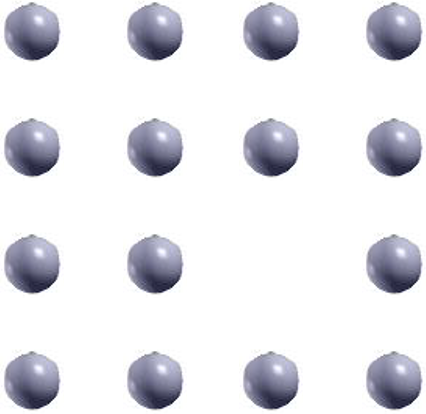
\includegraphics[height=1.2in]{Figs/Ch1/vacancy.png}
		\caption{Vacancy}
		\vspace*{1cm}
	\end{subfigure}%
	~ 
	\begin{subfigure}[t]{0.3\textwidth}
		\centering
		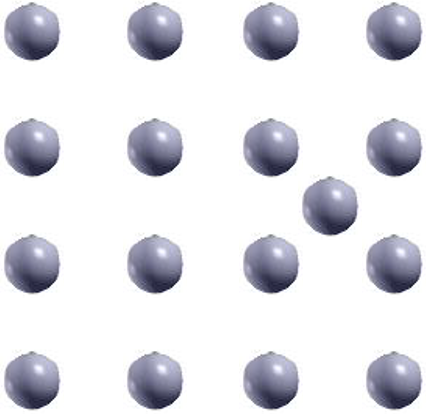
\includegraphics[height=1.2in]{Figs/Ch1/self-inter.png}
		\caption{Self-Interstitial}
	\end{subfigure}
	
	\begin{subfigure}[b]{0.3\textwidth}
		\centering
		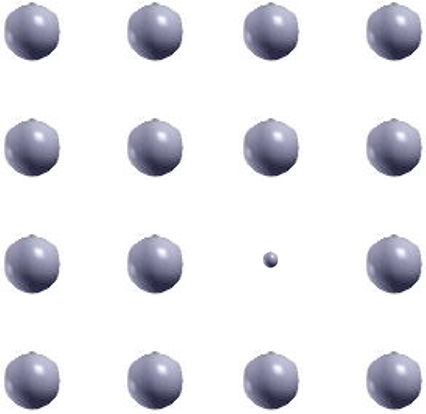
\includegraphics[height=1.2in]{Figs/Ch1/sub-impure.png}
		\caption{Substitutional Impurity}
	\end{subfigure}%
	~ 
	\begin{subfigure}[b]{0.3\textwidth}
		\centering
		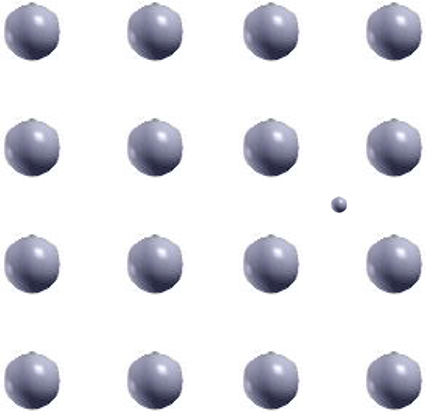
\includegraphics[height=1.2in]{Figs/Ch1/foreign.png}
		\caption{Foreign Interstitial}
	\end{subfigure}
	\caption{Point Defects:vacancy, self-interdtitial, substitutional impurity and foreign interstitial.}
	\label{1.6}
\end{figure}
\FloatBarrier
 Point defects are responsible for a plethora of deleterious effects at the device level in III-nitrides: they can reduce radiative efficiency, produce undesired luminescence act and as parasitic current paths \cite{Reshchikov2005}.
\subsubsection{1-D Defects}
Dislocations in GaN epilayers are categorised in two main forms: misfit dislocations (MDs) and threading dislocations (TDs). The origins of misfit dislocations are quite well understood: they occur through the release of misfit strain at interfaces between two crystals of differing lattice constants. The process is shown in Fig.\ref{1.7}: a film with a lattice parameter greater than the substrate is grown as is typical for III-nitride epilayers (GaN on sapphire or InGaN on GaN) and as a result the grown layer experiences compressive stress and forms pseudomorphic layer. The top layer is strained and matched to the lower layer due to its smaller lattice parameter. Strain relaxation occurs as the pseudomorphic relationship is broken when the top film reaches a critical thickness and results in the formation of misfit dislocations.

\begin{figure}
	\begin{subfigure}[b]{0.3\textwidth}
		\centering
		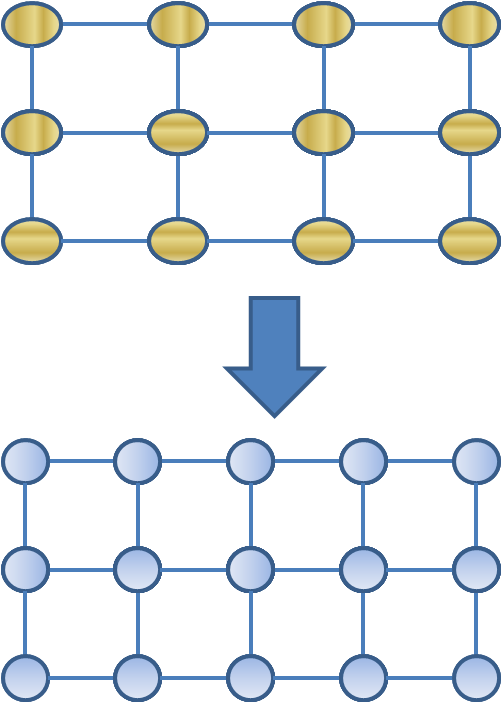
\includegraphics[width=.85\linewidth]{Figs/Ch1/MDa}
		\caption{}
	
	\end{subfigure}%
	\hspace*{0.5cm}
	\begin{subfigure}[b]{0.3\textwidth}
		\centering
		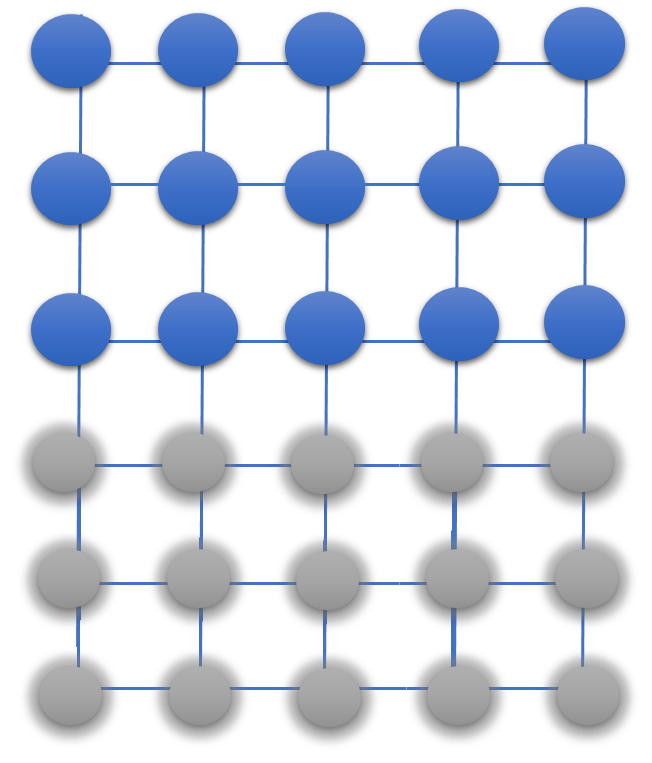
\includegraphics[width=.85\linewidth]{Figs/Ch1/MDb}
		\caption{}
		
	\end{subfigure}%
	\hspace*{0.5cm}
	\begin{subfigure}[b]{0.3\textwidth}
		\centering
		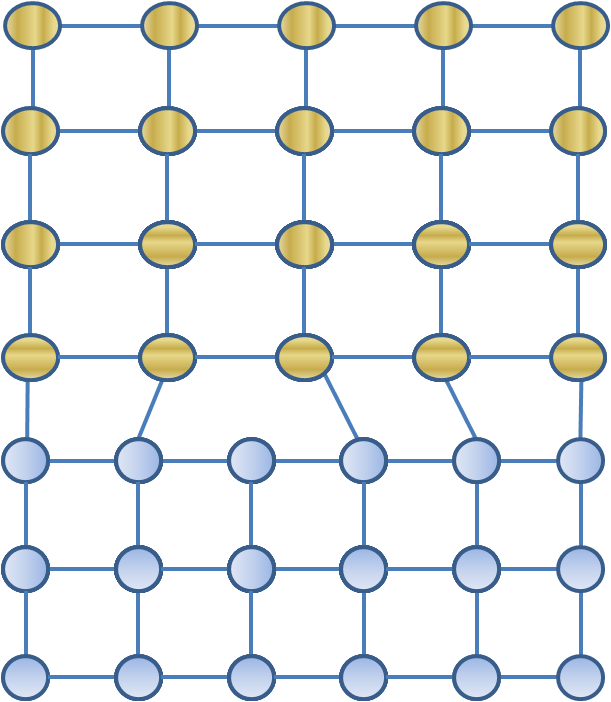
\includegraphics[width=.85\linewidth]{Figs/Ch1/MDc}
		\caption{}
	\end{subfigure}%

	\caption{Misfit dislocation formation through strain relaxation for heteroepitaxial growth: a) the film is grown on a substrate of smaller lattice size b) film maintains a pseudomorphic relationship with the substrate c) the film relaxes through the formation of a dislocation.}
\end{figure}
\FloatBarrier

The origins of TDs are far less well understood. TDs are not believed to relieve mismatch stress, and typically propagate perpendicular to the planar surface. TDs are classified into three categories based on their Burgers vector, as shown in Table.\ref{tab1.4}.

\begin{table}[h]
	\centering
	\begin{tabular}{p{4cm} p{4cm}   }
		\centering
		\textbf{Dislocation type}& \textbf{Burgers vector} \\
		\hline
		$\mathbf{a}$ type & $\frac{1}{3}<11\bar{2}0>$ \\
		$\mathbf{c}$ type& $<0001>$ \\
		$\mathbf{a+c}$ type & $\frac{1}{3}<11\bar{2}3>$ \\
		\hline
		
	\end{tabular}
	\caption{Burgers vectors for pure edge ($\mathbf{a}$), pure screw ($\mathbf{c}$) and mixed ($\mathbf{a+c}$)  TDs}
	\label{tab1.4}
\end{table}
\FloatBarrier

It was initially reported that GaN islands on sapphire during the initial stages of growth may be misorientated with respect to one another and that during the coalescence of these misorientated islands \cite{Ning1996}. This was seemingly disproven by a transmission electron microscopy data from a study on partially coalesced GaN on sapphire layers at various growth stages, which indicated the large majority of TDs seemed to initiate from within the nucleation layers at the GaN/sapphire interface rather than at coalescence boundaries. Oliver {\it et al}. used silane treatment to enlarge dislocation pits and observe them using atomic force microscopy, finding no significant relationship between boundary regions and the locations of dislocations \cite{Oliver2008a}. It was however suggested that dislocations may arise from the overgrowth of smaller islands by larger ones. Thus, while there is convincing evidence that TDs do not originate due to island coalescence, the actual mechanism behind their generation remains poorly understood.

\subsubsection{2-D Defects}

Stacking faults are defects which disrupt the regular stacking sequence of the crystal structure, in non-polar heterostructures they can intersect the QW layers. As a result of this, stacking faults are a more pressing concern than dislocations in epitaxial films grown along alternative directions to the {\it c}
-plane, as in polar materials stacking faults tend to remain in the nucleation layers \cite{Scholz2012}. Fig.\ref{1.7} shows different forms of stacking faults in $(11\bar{2}0)$ GaN ({\it a}-plane) on {\it r}-plane sapphire.  Basal-plane stacking faults \nomenclature[z-BSF]{BSF}{Basal-plane Stacking Fault} (BSFs) are atomic layers with a modified stacking sequence in the wurtzite crystal matrix. These BSFs can transfer to another stacking plane through prismatic stacking faults \nomenclature[z-PSF]{PSF}{Prismatic Stacking Fault} (PSFs). BSFs can also be bound by partial dislocations \nomenclature[z-PD]{PD}{Partial Dislocation} (PDs).


\begin{figure}[h]
	\begin{subfigure}[t]{0.4\textwidth}
	\centering
	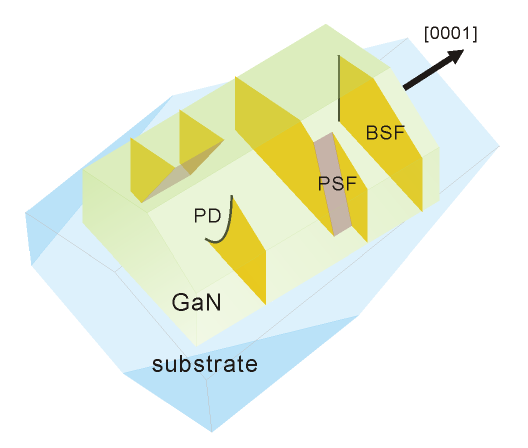
\includegraphics[width = 1\textwidth]{Figs/Ch1/bsf.png}
	\caption{}
	\end{subfigure}%
		\hspace*{1cm}
	~	
	\begin{subfigure}[t]{0.4\textwidth}
		\centering
		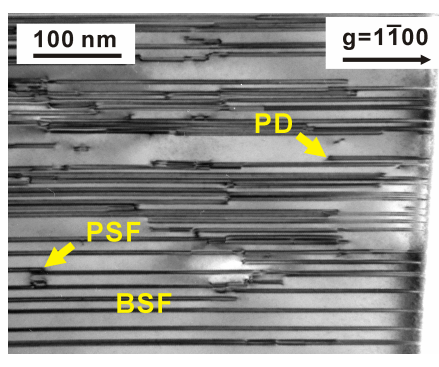
\includegraphics[width=1\textwidth]{Figs/Ch1/bsfTEM.png}
		\caption{}
	\end{subfigure}
	\caption {a) {\it a}-plane GaN showing basal plane stacking faults (BSFs), prismatic stacking faults (PSFs) and stacking faults bounded partial dislocations (PDs) shown schematically b) and in TEM. Adapted from \cite{Liu2011}.}
	\label{1.7}
\end{figure}
\FloatBarrier

Three types of BSFs exist in wurtzite crystals, they are classified based on their displacement vector $\mathbf{\vv{R}}$ as shown in Table.\ref{tab1.5}.

\begin{table}[h]
	\centering
	\begin{tabular}{cc}
		\centering
		\textbf{BSF type}& \textbf{Displacement vector $\mathbf{\vv{R}}$ } \\
		\hline
		$I_{1}$  & $\frac{1}{6}<20\bar{2}3>$ \\
		$I_{2}$ & $\frac{1}{3}<10\bar{1}0>$ \\
		$E$  & $\frac{1}{2}<0001>$ \\
		\hline
		
	\end{tabular}
	\caption{BSF types in wurtzite materials.}
	\label{tab1.5}
\end{table}
\FloatBarrier

Whilst TDs are considered completely undesirable due to the adverse effects they may have on radiative processes and carrier transport, it has been suggested the presence of BSFs on the optical properties may be beneficial in some cases. Indeed, BSFs have been shown to enable radiative recombination through confinement and thus act as QWs with an exciton binding energy of 45 meV \cite{Rebane1997}.

\subsubsection{3-D Defects}

There are many forms of 3-D defects in III-nitrides such as voids, nanopipes and cracks. In this particlar section we will focus on those relevant to the work featured in later chapters of this work.\\
Inverted hexagonal pyramid defects, also known as V-pits, are defects commonly found at the surface of InGaN/GaN QW structures. They form as a result of a TD intersecting the QW layers. It is believed that the low temperatures required for the growth of the InGaN layers allow even minute perturbations of the surface to persist into inclined facets with low growth rates, such as the $(1\bar{1}01)$ facets. The apex of TDs thus provide optimal conditions for the formation of V-pits during the growth of InGaN layers \cite{Hangleiter2005}. Interestingly, TEM studies have shown that the QW layers disrupted by the defect grow along the semi-polar facets at a lower thickness \cite{Hangleiter2005,Han2013,Tsai2007}. Fig.\ref{1.8} shows a TEM image of a V-pit in an InGaN/GaN multiple QW structure with a schematic describing this defect and how it affects the growth of the QWs.

\begin{figure}[h]
	\centering
	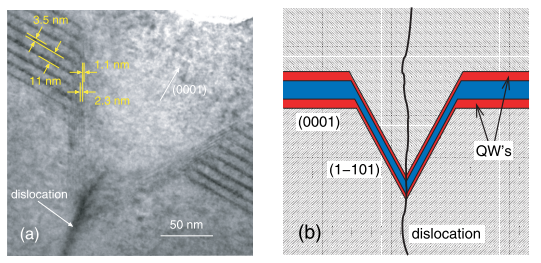
\includegraphics[width=0.7\textwidth]{Figs/Ch1/vpit.png}
	\caption {a) TEM image of a hexagonal inverted pyramid defect b) Schematic  of a V-pit with its associated TD \cite{Hangleiter2005}.}
	\label{1.8}
\end{figure}
\FloatBarrier 

The existence of TDs as non-radiative recombination centres has been well documented \cite{Bennett2010b}, however it is believed that V-pits suppress this non-radiative recombination and provide an increase in light emission efficiency in III-nitride devices by providing an energy barrier surround TDs \cite{Hangleiter2005}. Hangleiter {\it et al}. suggested the thinner wells grown along the semi-polar facets of the V-pit provided an energy barrier of several hundred meV relative to the normal {\it c}-plane QWs \cite{Hangleiter2005}, thus providing a potential landscape shielding carriers from TDs, as shown in Fig.\ref{1.9}.

\begin{figure}[h]
	\centering
	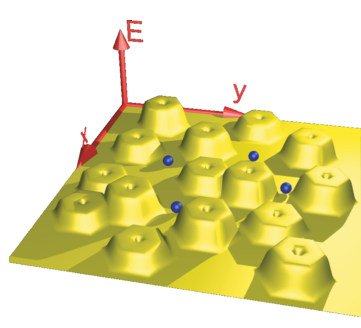
\includegraphics[width=0.5\textwidth]{Figs/Ch1/landscape.png}
	\caption {Potential landscape due to V-pits decorating the apex of TDs: carriers (blue) need to overcome the energy barriers to recombine non-radiatively at the TDs \cite{Hangleiter2005}.}
	\label{1.9}
\end{figure}
\FloatBarrier 

 
%********************************** %Second Section  **************************************
\section{III-nitride Devices } %Section - 1.1 
\subsection{Light Emitting Diodes}
Light emitting diodes (LEDs) are the most common application of III-nitride materials. These devices typically consist of a {p-n} junction. This consists of material containing excess acceptor ({\it p}-doped) and another containing excess donor impurities ({\it n}-doped) which are brought into contact. This allows holes from the {\it p}-type material and electrons from the {\it n}-type material to diffuse across the junction until an equilibrium state is reached, a region where the electric field from the charged dopants on either side prevents diffusion is formed known as the depletion region. The application of forward bias reduces the built-in potential across the depletion region and allows for the flow of electrons and holes across the junction, as shown schematically in Fig.\ref{1.10}.
\begin{figure}[h]
		\hspace*{1cm}
	\begin{subfigure}[t]{0.4\textwidth}
		\centering
		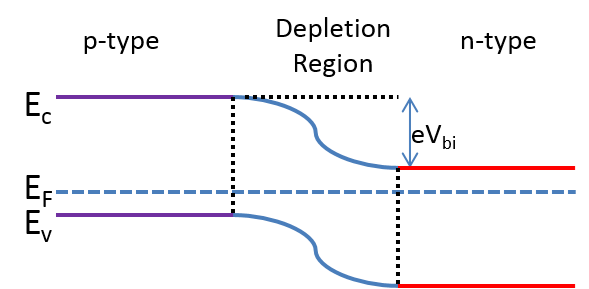
\includegraphics[width = 1\textwidth]{Figs/Ch1/pn1.png}
		\caption{}
	\end{subfigure}%
	\hspace*{1cm}
	~	
	\begin{subfigure}[t]{0.4\textwidth}
		\centering
		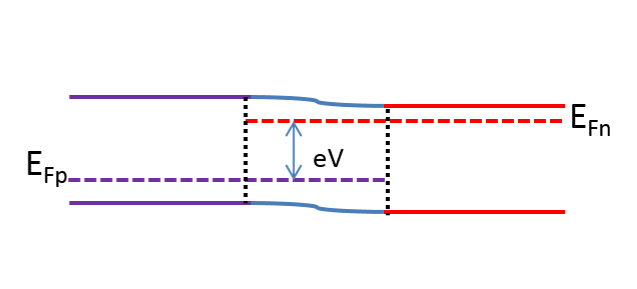
\includegraphics[width=1\textwidth]{Figs/Ch1/pn2.png}
		\caption{}
	\end{subfigure}
	\caption {a) {\it p-n} junction at equilibrium, with the conduction band, Fermi level and valence band denoted $E_{c},E_{F}$ and $E_{v}$ respectively, the built in potential across the junction is denoted as $V_{bi}$ b) under forward bias of V.}
	\label{1.10}
\end{figure}
\FloatBarrier

A schematic of a general LED structure is shown in Fig.\ref{1.11}. Visible light LED structures typically contain a magnesium doped {\it p}-region and a silicon doped {\it n}-region. An electron blocking layer \nomenclature[z-EBL]{EBL}{Electron Blocking Layer} (EBL) consisting of a material with a higher bandgap than GaN ( in this case AlGaN) is used to prevent the leakage of electrons into the {\it p}-doped region and confine them in the InGaN QW active region.

\begin{figure}[h]
	\centering
	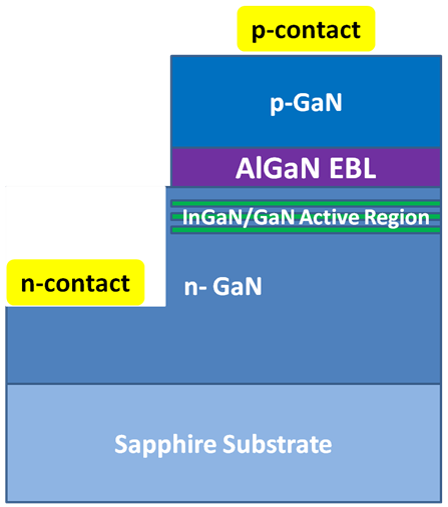
\includegraphics[width=0.3\textwidth]{Figs/Ch1/led.png}
	\caption {Typical visible light LED structure grown on a sapphire substrate \cite{Ren2015}.}
	\label{1.11}
\end{figure}
\FloatBarrier 

\subsection{Microcavities}

Microcavity emitters possess rather singular optical properties due to their dimensions. By matching one or more dimensions of the cavity to the order of the wavelength of confined light a plethora of effects can be produced such as low-threshold lasing, directional luminescence and enhanced nonlinear conversion \cite{Christopoulos2007}. By confining a dipole within a microcavity, one can modify its emissive properties by altering the photon density of states. The interaction rate between the confined dipole and a cavity photon relative to the average rate of dissipation of a cavity determines whether the microcavity operates in the weak-coupling or strong-coupling regime.\\Weak coupling occurs when dissipation overwhelms the dipole-cavity photon interaction: in essence, the effect of the microcavity in this case is to alter the vacuum description of the dipole lifetime, resulting in an increase in spontaneous emission for on-resonance cavity modes, known as the Purcell effect \cite{Vahala2003}. Weakly-coupled microcavity systems have applications across a wide range of optoelectronic devices due to this effect: from enhancing the recombination rate and extraction efficiency of embedded single photon emitters \cite{Jarjour2007a} to the development of high efficiency, low threshold lasers \cite{Aharonovich2013}.\\An interaction occurring on shorter timescales than the average dissipation rate of the cavity photon is defined as being in the strong coupling regime, and results in the formation of admixed eigenstates populated by quasiparticles known as polaritons, which are hybrid particles combining a photon and an electric dipole. The bosonic nature of these quasiparticles has led to the observation of spontaneously emitted coherent light from condensates of exciton-polaritons,  a phenomenon also known as polariton lasing \cite{Malpuech2002}. The expected threshold energy for coherent emission from a polariton laser is expected to be much smaller than that of a conventional laser due to the lack of the requirement of population inversion , thus rendering polariton lasers extremely attractive as low-threshold lasing applications \cite{Christopoulos2007}. Beyond polariton lasing, strong coupling in microcavities is also required for key quantum information processing tasks such as the entanglement of distinguishable quantum systems and controlled coherent coupling \cite{Imamoglu1999,Hennessy2007}.

\subsubsection{Cavity Parameters and Design}
The ability of a microcavity to confine light is thus a crucial parameter in producing the required effects and is known as the cavity 'quality factor' which is described by Eq.~\ref{Q-fac}.

\begin{equation}\label{Q-fac}
Q = \frac{\nu_{0}}{\delta\nu_{0}}
\end{equation}

Where $\nu_{0}$ is the resonant frequency of the cavity mode and $\delta\nu_{0}$ is the mode bandwidth. Cavity quality factor can be understood as a parameter describing the rate of energy decay the resonant mode undergoes within the cavity and thus may be alternatively described using an exponential characteristic decay constant $\tau_{cav}$ as shown in Eq.\ref{exp}, where $Q^{-1}$ is the proportion of energy lost during a single cavity round-trip.

\begin{equation}\label{exp}
Q = \pi\tau_{cav} \nu_{0}
\end{equation}

The manner in which the resonant mode fields interact with the cavity geometry is also determined by the effective modal volume of the cavity, which is described by Eq.\ref{mode}.

\begin{equation}\label{mode}
V_{eff}= \int_{V}\frac{\epsilon_{0}(\mathbf{r})|\mathbf{E}(\mathbf{r})|^{2}}{max[\epsilon_{0}(\mathbf{r})|\mathbf{E}(\mathbf{r})|^{2}]}dV
\end{equation}

where $|\mathbf{E}(\mathbf{r})|^{2}$ is the normalised electric field amplitude, $\epsilon_{0}$ is the dielectric constant and V is the quantization volume. $V_{eff}$ describes the manner in which cavity supports the distribution of the resonant mode, thus in some cases a large evanescent field component must be included in the calculation of the modal volume.
\\ Cavities often support more than one optical mode, which gives rise to another parameter, known as the free spectral range \nomenclature[z-FSR]{FSR}{Free Spectral Range} (FSR), which is defined as the frequency spacing between successive resonant modes. This parameter is crucial to lasing cavities as the probability of photon into a lasing mode is affected by the number of modes supported by the cavity. The FSR as well as parameters needed to define cavity quality factor are shown schematically in Fig.\ref{1.12}. 

\begin{figure}[h]
	\centering
	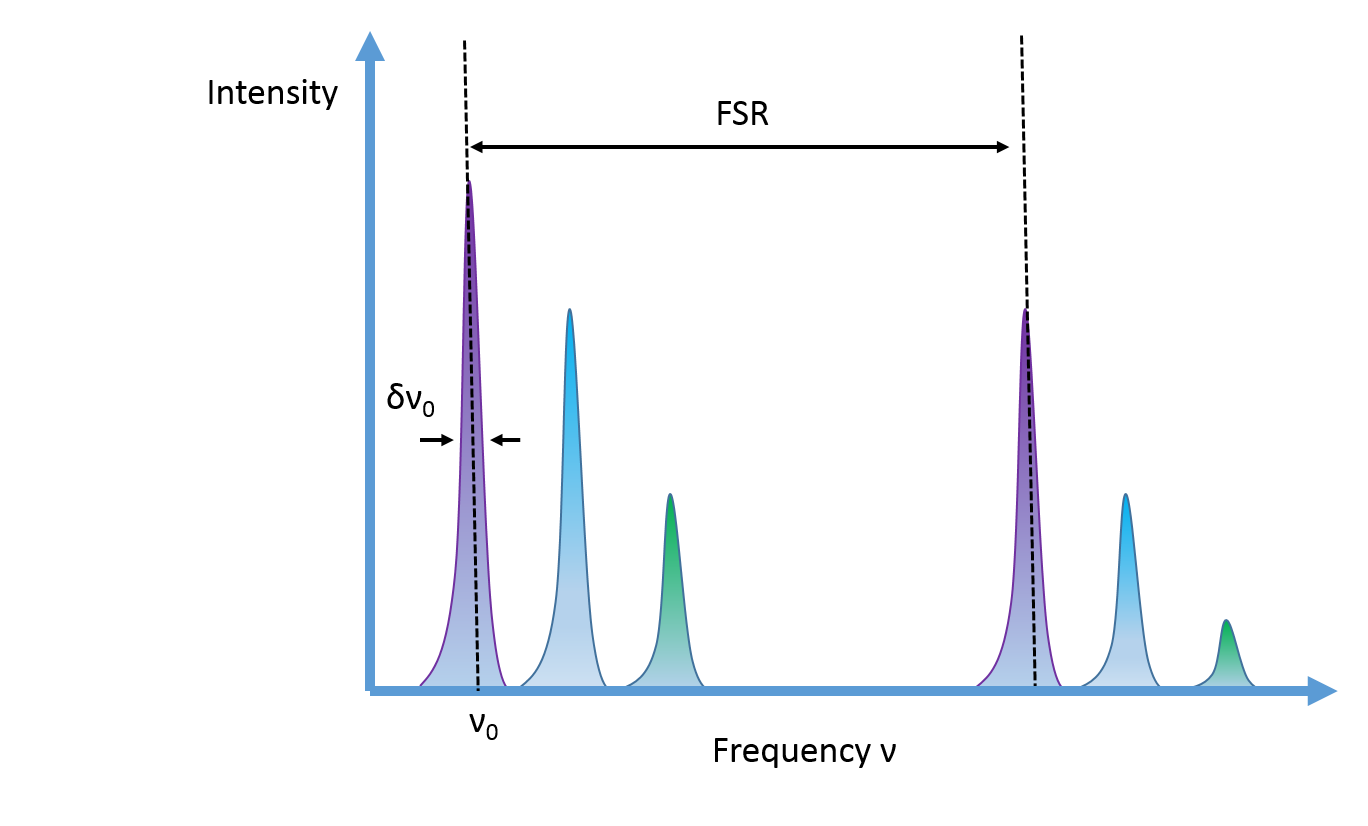
\includegraphics[width=0.9\textwidth]{Figs/Ch1/modes.png}
	\caption {Illustration of the some key parameters such as FSR and resonant cavity mode FWHM. }
	\label{1.12}
\end{figure}
\FloatBarrier 


Cavities modify the optical density of states of an emitter through the generation of standing electromagnetic waves. There are several manners through which to achieve this: at the most basic level an optical cavity is a set of single reflective interfaces, spaced at a specific distance designed to enhance a particular optical mode. However, many cavity designs which employ the use of refractive index mismatches for total internal reflection or an array of boundaries leading to interference enhanced optical modes also exist, as shown in Fig.\ref{1.13}.
\begin{figure}
	\begin{subfigure}[b]{0.3\textwidth}
		\centering
		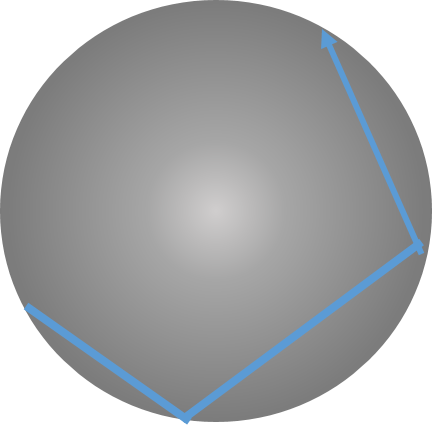
\includegraphics[width=.75\linewidth]{Figs/Ch1/mdisk}
		\caption{Total internal reflection}
		
	\end{subfigure}%
	\hspace*{0.5cm}
	\begin{subfigure}[b]{0.3\textwidth}
		\centering
		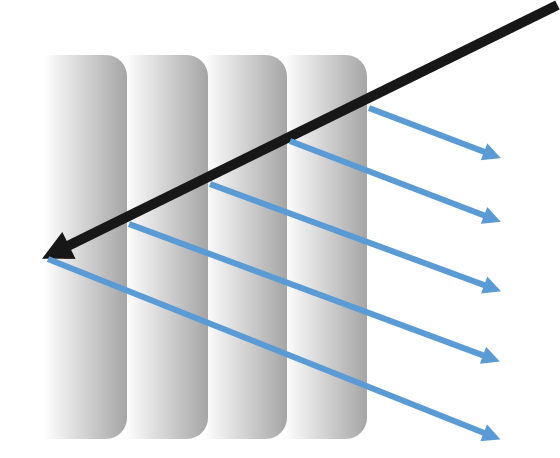
\includegraphics[width=.85\linewidth]{Figs/Ch1/dbr}
		\caption{1-D interference}
		
	\end{subfigure}%
	\hspace*{0.5cm}
	\begin{subfigure}[b]{0.3\textwidth}
		\centering
		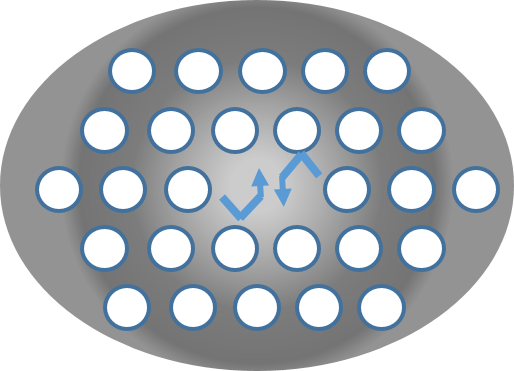
\includegraphics[width=.85\linewidth]{Figs/Ch1/pcc}
		\caption{2-D interference}
	\end{subfigure}%
	
	\caption{Optical resonators.}
	\label{1.13}
\end{figure}

\FloatBarrier

\subsubsection{Microdisk Cavities}

Total internal reflection can be exploited in circular geometries such as microdisk/ring/sphere devices, in which whispering gallery modes \nomenclature[z-WGM]{WGM}{Whispering Gallery Mode} (WGMs) propagate around the periphery of the disk.\\
Microdisks can be described as a cylinder of with a low height:radius ratio supported by a pillar of a small radius ( less than half of the cylinder). The position of the WGMs is described by Snell's law: only light satisfying the condition described by Eq.\ref{eq1} is contained within the microdisk due to internal reflection.

\begin{equation} \label{eq1}
\theta_{c}=sin^{-1}(\frac{n_{2}}{n_{1}})
\end{equation}

Assuming the microdisk thickness is small enough to act as a waveguide in the vertical direction, we can consider the propagation of a ray of light in 2-D as in Fig.\ref{1.14}. The forbidden position of the WGMs as defined by Eq.\ref{eq1} is given by $R_{min}$.
\begin{figure}[h]
	\centering
	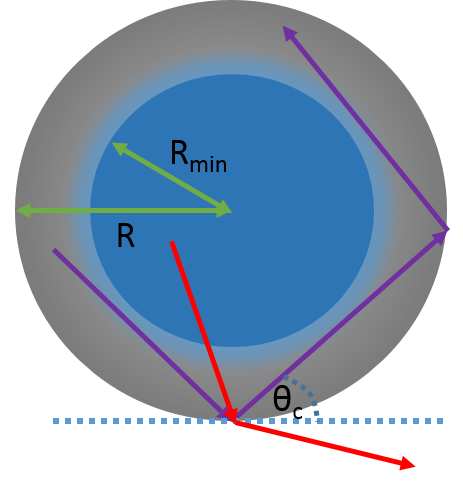
\includegraphics[width=0.5\textwidth]{Figs/Ch1/mdiskray.png}
	\caption {Illustration of the minimum radius $R_{min}$ for WGM propagation. Rays traversing the region $r<R_{min}$ (denoted in red) exceed the critical angle $\theta_{c}$ and thus escape the cavity. Rays travelling outside this region $r>R_{min}$ (denoted in violet) are confined.  }
	\label{1.14}
\end{figure}
\FloatBarrier 
Thus the fabrication of microdisks relies heavily on the ability to 'undercut' the microdisk material whilst still leaving a pedestal, as shown in Fig.\ref{1.15}. This is a particularly difficult problem to address in terms of III-nitride materials due to the excellent thermal ande chemical stability of GaN.  Early efforts in microdisk nitride fabrication involved dry-etching processes, utilising the refractive index mismatch between the light emitting GaN layers and the sapphire substrate to confine light \cite{Tamboli2007}. Although stimulated emission and lasing was observed by Chang {\it et al}. in dry-etched GaN microdisk cavities \cite{Chang1999}, Haberer {\it et al}. \cite{Haberer2004} reduced the required excitation power densities for lasing by an order of magnitude by employing photoelectrochemical (PEC) etching to undercut GaN microdisks, thus providing superior optical confinement due to the index contrast of the GaN/air interface  relative to the GaN/sapphire interface used by Chang {\it et al}. \cite{Chang1999}. Further improvements in fabrication were achieved by Tamboli et al. with room temperature lasing achieved in GaN/InGaN microdisks through enhancements in microdisk circularity and sidewall smoothness \cite{Tamboli2007}. 
\begin{figure}[h]
	\centering
	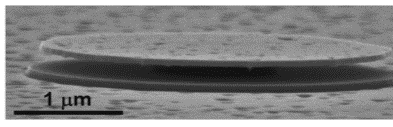
\includegraphics[width=0.5\textwidth]{Figs/Ch1/mdisksem.png}
	\caption {Scanning electron microscope image of a GaN microdisk produced by selective etching of sacrificial AlInN layers \cite{Simeonov2008}.}
	\label{1.15}
\end{figure}
\FloatBarrier 


\subsubsection{Nanobeam Cavities}

Photonic crystals are periodic structures which affect photons in an manner analogous to the way atomic lattices affect electrons in solids. They can be considered as artificial materials exhibiting a dielectric function which varies periodicially in either one, two or three dimensions. The principal mechanism of light confinement in this case is known as distributed bragg reflection as is shown in Fig.\ref{1.13}b).\\
Whilst micro-toroid and microdisk cavities have the potential to achieve extremely high Q-factors many applications which involve strong coupling, non-linear optical processes and spontaneous emission and other similar processes require a high ratio between the Q-factor and the effective modal volume ($V_{eff}$). This figure of merit can be achieved in travelling-wave cavity geometries due to the potential for extremely small modal volumes. Yablonovitch \cite{Yablonovitch1987} and John \cite{John1987} first proposed the design of 3-D photonic crystal cavities which in theory would possess ultra-high Q-factors, minute modal volumes and perfect reflectivity in all directions. Despite the extremely promising theoretical properties of 3-D photonic crystal cavities, their fabrication has proven to be particularly challenging with few demonstrations of high-Q 3-D PCCs reported in literature \cite{Ishizaki2013}, \cite{Tandaechanurat2011}. PCCs of lower dimensionality are thus prime candidates for practical applications due to fewer (though not vanishing!) fabrication issues. In particular 1-D PCCs such as suspended structures known as nanobeams are extremely promising due their ability to realise of high-Q, low $V_{eff}$ cavities even in low index materials such as $SiO_{2}$ \cite{Gong2010}. For these reasons we will specifically be considering 1-D photonic crystal cavities in the nanobeam geometry in this work.\\
Electromagnetic field confinement is achieved in nanobeam structures by Bragg scattering from the photonic crystal in one direction, and index guiding in the other two directions. A nanobeam can essentially be considered as a wavelength-scale Fabry-Perot cavity with photonic crystal mirrors \cite{Deotare2009}: as the nanobeam waveguide mode is trapped and reflected by these mirrors, it also penetrates some distance into them. If the fields terminate at the mirror boundaries, this would lead to large scattering losses due to the large impedance mismatch \cite{Notomi2008}. In order to avoid this impedance mismatch between the waveguide mode and the Bloch mode of the mirror, the photonic crystal mirrors are tapered in order to match the evanescent mirror Bloch mode \cite{Lalanne2003} as shown in Fig.\ref{1.16}.


\begin{figure}[h]
	\centering
	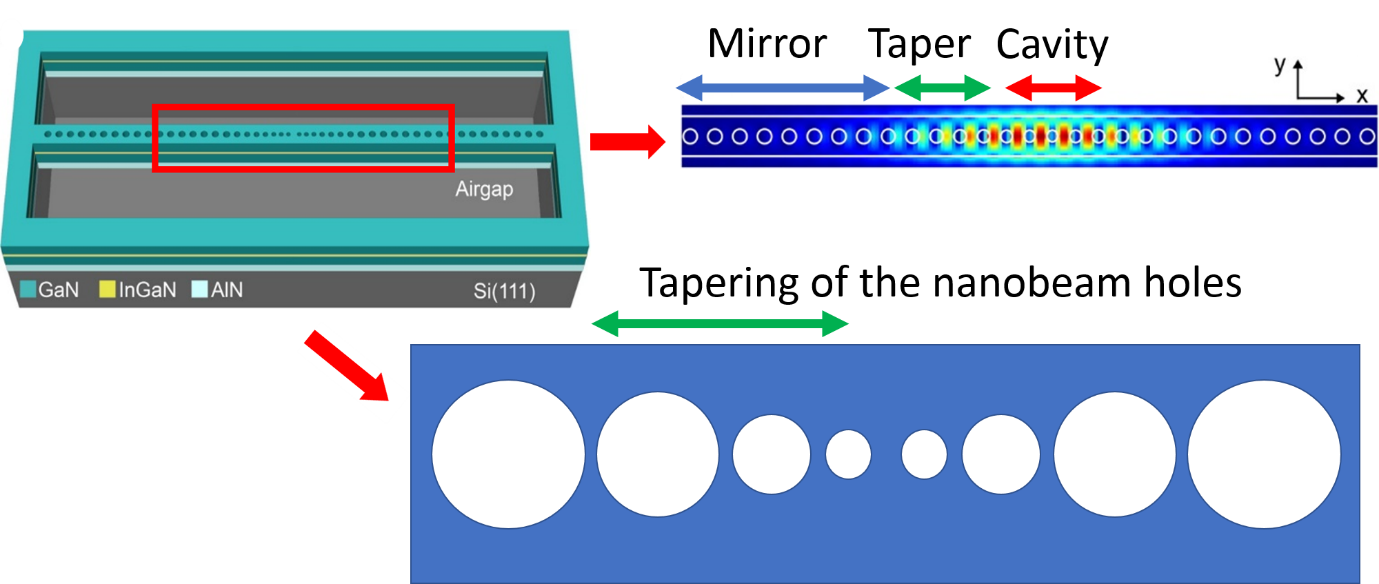
\includegraphics[width=0.9\textwidth]{Figs/Ch1/nb1.png}
	\caption {Nanobeam schematic and 3-D FDTD simulation of the electric field intensity profile of the cavity mode adapted from \cite{Trivino2015}. }
	\label{1.16}
\end{figure}
\FloatBarrier 

\subsection{Nanowires}
The lack of readily available, low-cost substrates for the epitaxial growth of GaN and its associated alloys has motivated research into the growth of III-nitrides in nanowire geometries. Indeed, studies have shown that epitaxial GaN nanowires can be grown with far lower dislocation densities relative to bulk GaN due to a large surface-to-volume ratio. Furthermore, QWs grown radially along the non-polar facets of nanowires allow for the reduction of the polarization fields which can deleteriously affect the optical properties of polar III-nitride emitters without the need for expensive non-polar substrates. Furthermore, axial heterostructure nanowire geometries allow for the growth of {\it p-n} junctions within a single nanowire, allowing for the use of III-nitride nanowires as fundamental electrical components in optoelectronics. As such III-nitride nanowires have been utilised to develop high efficiency LEDs, electrically pump lasers with extremely low lasing thresholds and single photon sources with site-controlled QDs.

\begin{figure}

	\begin{subfigure}[b]{0.49\textwidth}
		\centering
		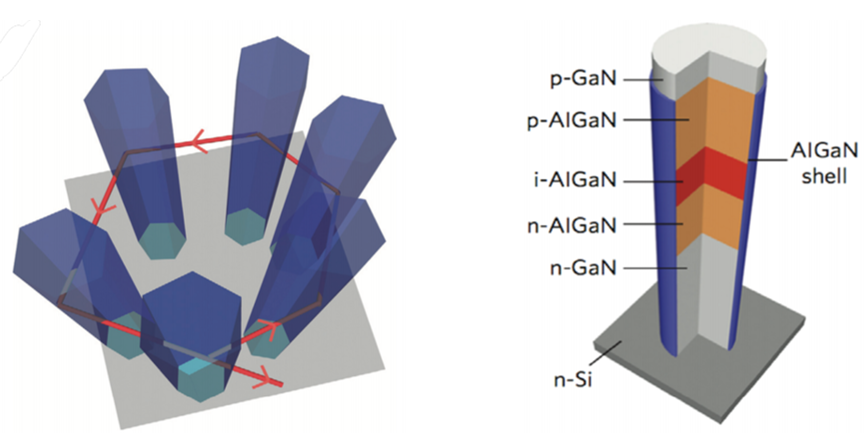
\includegraphics[width=.95\linewidth]{Figs/Ch1/Nwlaser.png}
		\caption{Axial GaN/AlGaN heterostructure nanowire for random lasing\cite{Li2015}}
		
	\end{subfigure}%
	\hspace*{0.5cm}
	\begin{subfigure}[b]{0.49\textwidth}
		\centering
		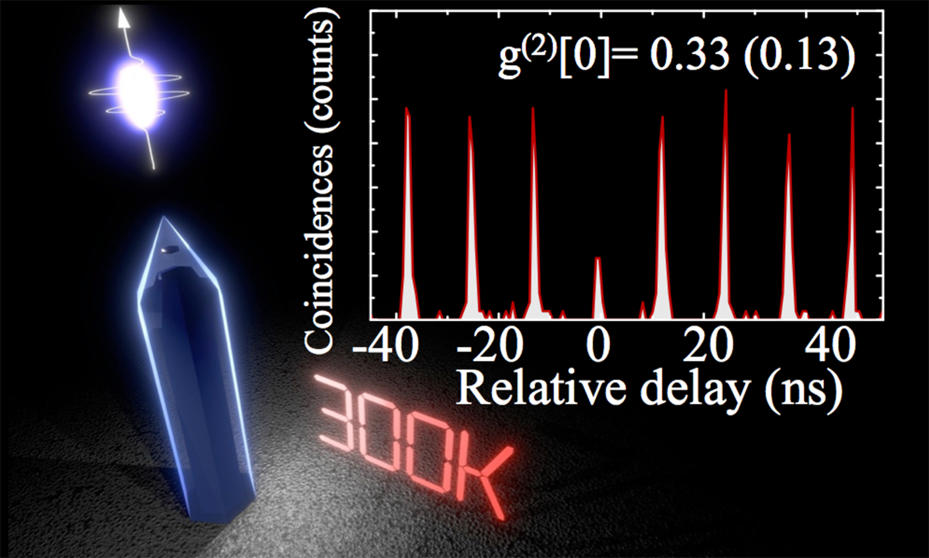
\includegraphics[width=.85\linewidth]{Figs/Ch1/holmes.png}
		\caption{Site-controlled QD in a GaN nanowire showing photon anti-bunching emission at room temperature \cite{Holmes2014}.}
	\end{subfigure}%
	
	\caption{III-Nitride nanowire applications.}
	\label{1.19}
\end{figure}

\FloatBarrier
